\begin{figure}[H]
  \centering
  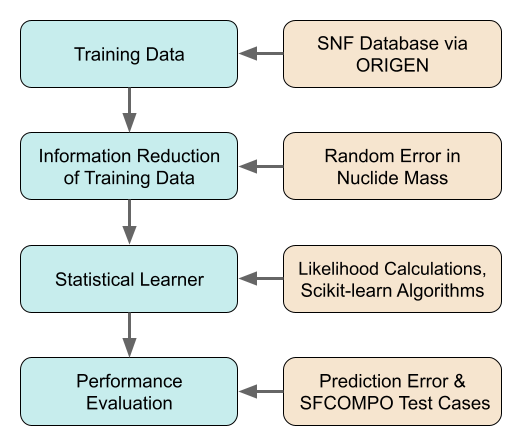
\includegraphics[width=0.7\linewidth]{./chapters/exp1/methodology1.png}
  \caption{First portion of the flowchart from Figure \ref{fig:method} being 
           described in this section.}
\end{figure}

\todo[inline]{intro, these nucs are chosen because they are radionuclides with
long enough half-lives}

In the second experiment, activities of radionuclides are necessary to
calculate gamma spectra from these values.

\begin{table}[!htb]
  \centering
  \begin{tabular}{@{}|l|l|l|l|l|l|l|l|@{}}
    \hline
    Ac227&\textbf{Am241}&\textbf{Am243}&Ba133&Cf249         &Cf252          &Cm243         &\textbf{Cm244} \\ \hline
    Cm245&\textbf{Cs134}&\textbf{Cs137}&Eu152&\textbf{Eu154}&Ho166m         &Kr85          &Nb94           \\ \hline
    Np236&\textbf{Np237}&Pa231         &Pm146&Pu236         &\textbf{Pu238} &\textbf{Pu239}&\textbf{Pu240} \\ \hline
    Ra226&Sb125         &Th228         &Th229&U232          & U233          &\textbf{U234} &\textbf{U235}  \\ \hline
  \end{tabular}
  \caption{Set of features saved for the second experiment, nuclide activities
           measured in $Curies$. The bold nuclide activities overlap with the 
           nuclides in Table \ref{tbl:nucmass}.}
  \label{tbl:nucacts}
\end{table}

The second feature set with the 32 nuclide activities listed in Table
\ref{tbl:nucacts} was designed with the following reasons in mind. First,
nuclide activities are the most straightforward units to use for application to
the \gls{DRF} in the \gls{GADRAS} tool for the second experiment. This process
is used to obtain gamma spectra for each \gls{SNF} entry in the database, which
is detailed in \ref{sec:inforeduc2}.  Second, these specific nuclides were
chosen because they fulfill four steps of filtering:
\begin{enumerate}
  \item They exist in the 196-long radionuclide list in \gls{GADRAS}.
  \item They have an activity above $1e-7\:Ci$ (cutoff chosen to filter out
  nuclides that are unlikely to produce gamma energy peaks).
  \item They have a half-life longer than $1\:year$ (cutoff chosen based on
  maximum cooling time of $16\:years$).
  \item They have at least one gamma energy line above $200\:keV$ (cutoff
  chosen based on low-energy gamma energy peaks being difficult to discern in
  some detectors).
\end{enumerate}

